\documentclass[paper=a4, fontsize=12pt]{article}

\usepackage[english]{babel}															% English language/hyphenation
\usepackage[protrusion=true,expansion=true]{microtype}				% Better typography
\usepackage{amsmath,amsfonts,amsthm}										% Math packages
\usepackage[pdftex]{graphicx}														% Enable pdflatex
\usepackage{color}													% If you use color and/or transparency
\usepackage[hang, small,labelfont=bf,up,textfont=it,up]{caption}	% Custom captions under/above floats		
\usepackage{url}
\usepackage[section]{placeins}
\usepackage[numbers]{natbib}

\title{random infrastructure networks (of networks)}

\begin{document}

\maketitle

\tableofcontents

\section{Conclusions for Power Grid Topologies}

\subsection*{Growth Process of (National) Grids}

\begin{itemize}
\item[start] many small-scale local networks on LV/MV \cite{50Hertz, BURN}
\item[update 1] if network's capacity becomes a limiting factor MV lines are extended
\item[update 2] HV overlay added, connecting also different local network on lower voltage \cite[p.3]{Lakervi1995}
\item[constraint] HV/EHV usually fulfill N-1 criterium \cite[p.7]{Lakervi1995}
\item[remark 1] Historically, EHV superseded HV in this role, but they still coexist. \cite[p.148]{Lakervi1995}
\item[remark 2] LV network growth driven by amount of load
\item[location] HV/MV substations close to load centres \cite[p.152]{Lakervi1995}
\end{itemize}

I hypothesise that it is probably sufficient to model three distinct network levels:
\begin{enumerate}
\item low,  LV, i.e. connecting all households in a building block to the next higher level
\item middle,  MV+HV, the actual distribution backbone in an area
\item high,  EHV, connecting different areas over long distances
\end{enumerate}

The low network grows radially from single nodes in the middle network proportional to the load development.
The high network consists of long-range connections with high capacity (and is the only one that is meshed ?).

The middle layer is maybe similar road networks \cite{Strano2012} in their construction?

\subsection*{Interconnections Between Different Countries/Regions}

Power grids are often interconnected via short AC/DC/AC lines and in general at EHV \cite[p.6]{Lakervi1995}.

\subsection*{Network Structure in General}

\begin{figure}
\centering
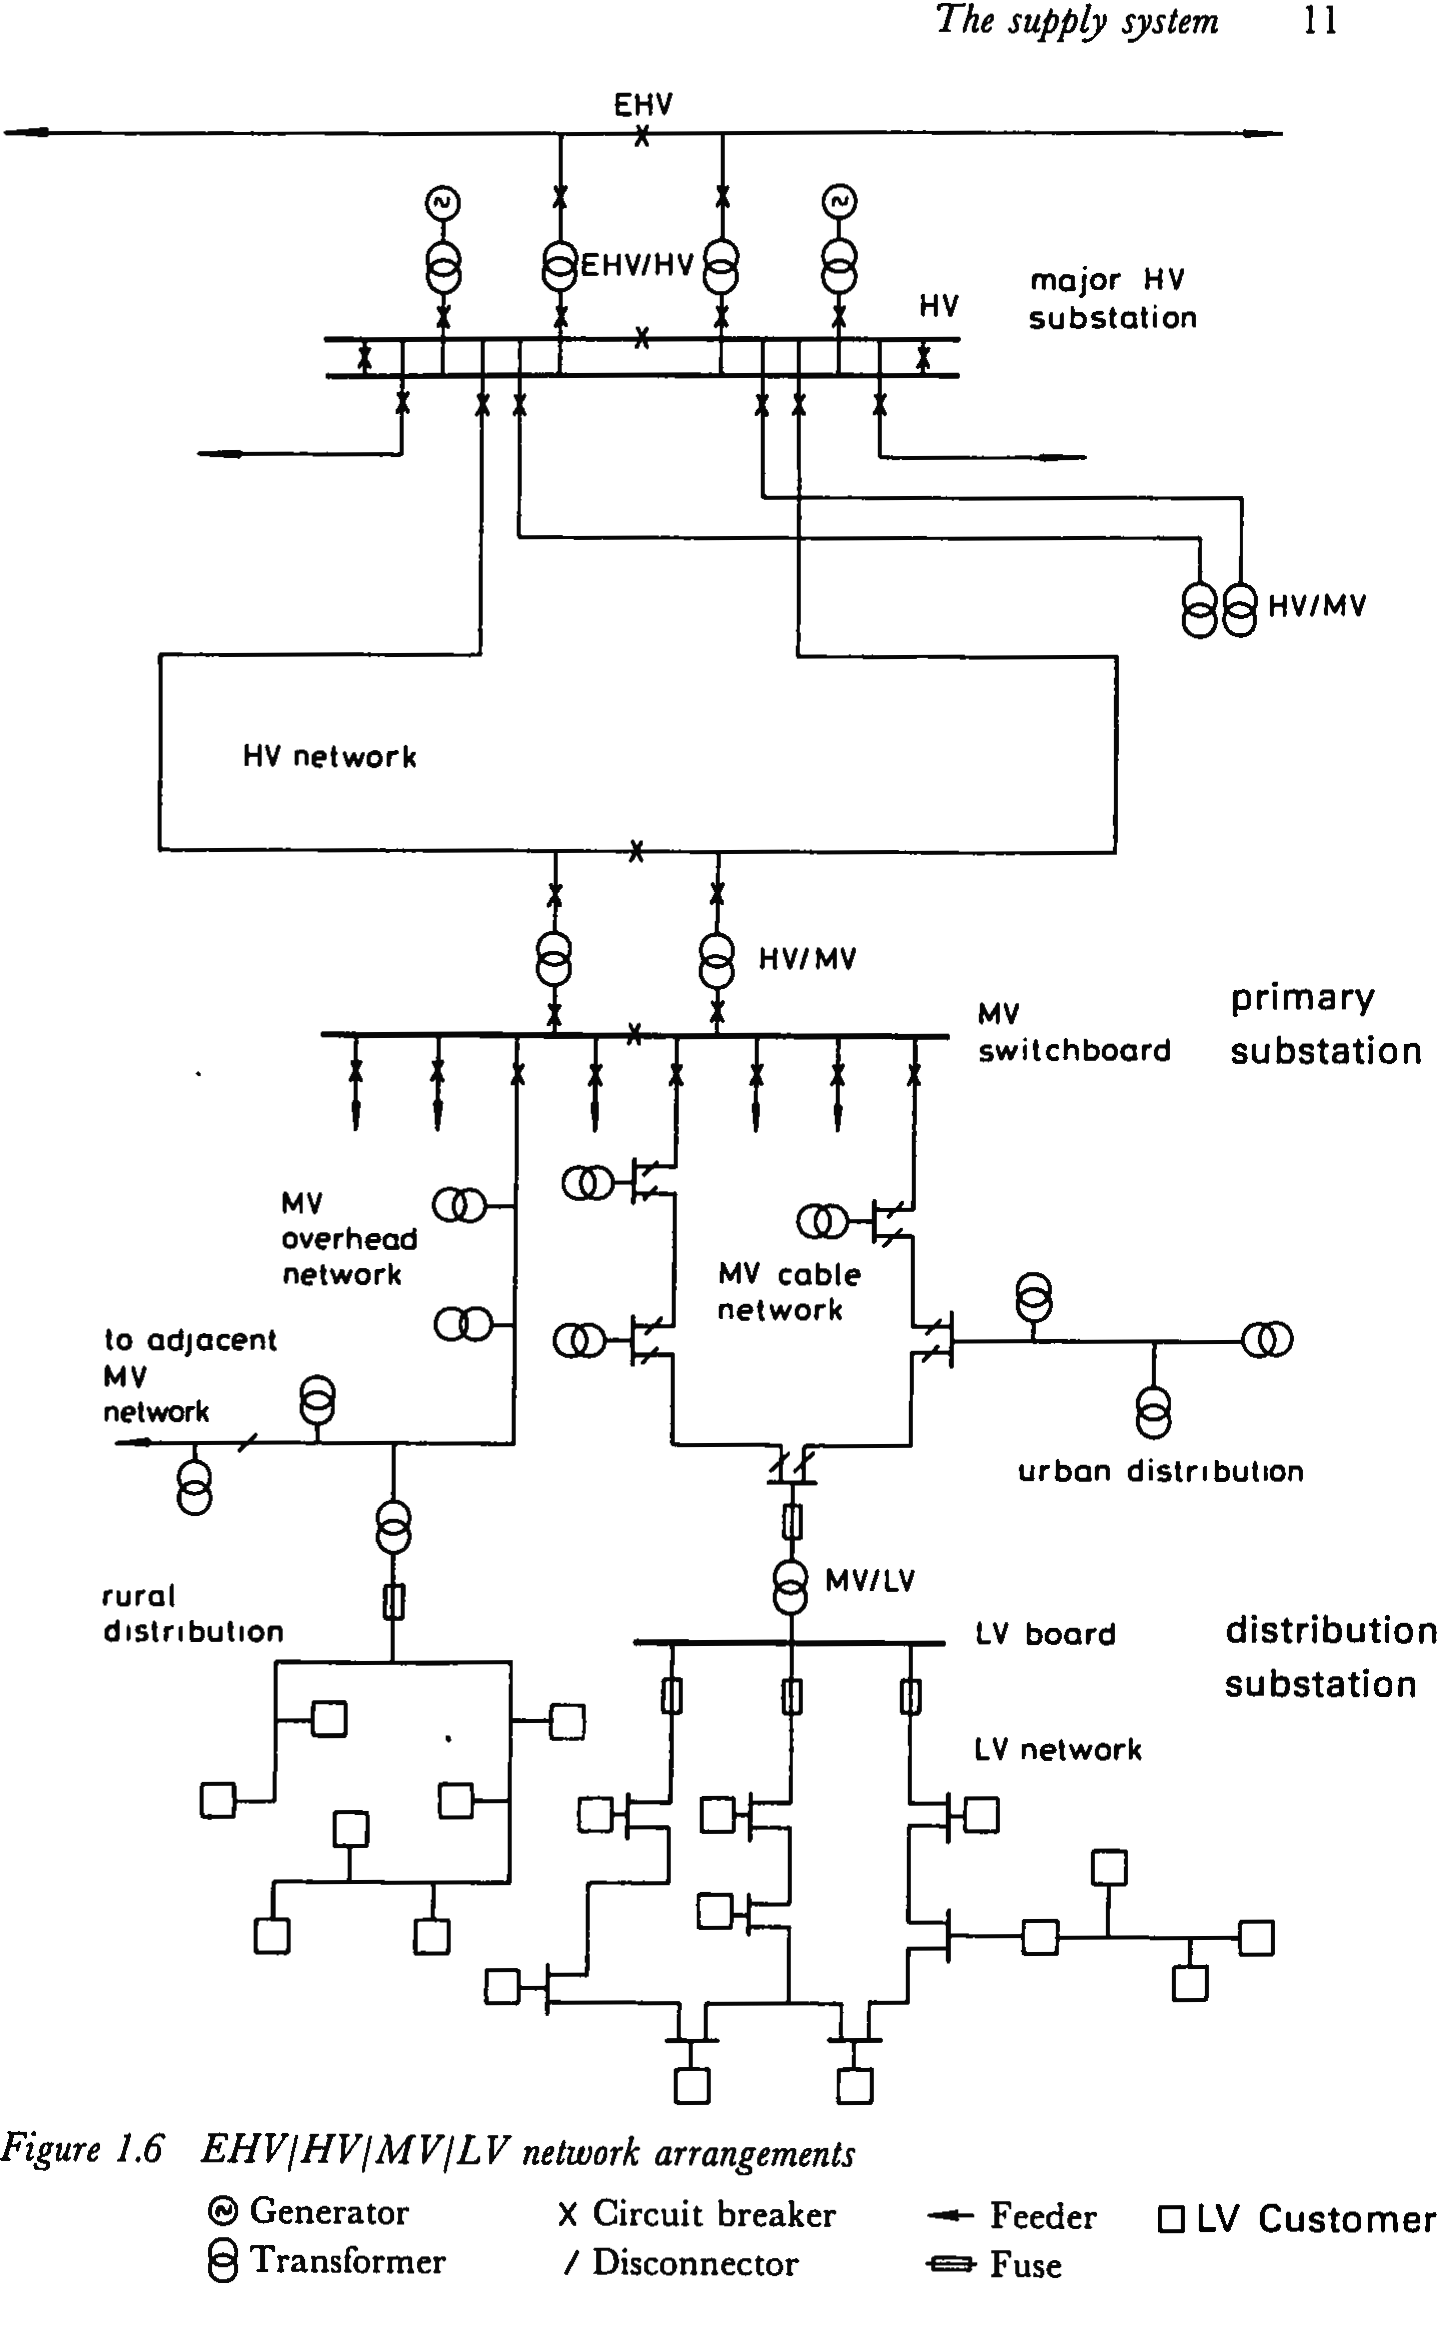
\includegraphics[height=\textheight]{lakervi-fig1p6.png}
\caption{Fig. 1.6 from \cite{Lakervi1995}.}
\end{figure}

\begin{itemize}
\item[HV] typically built as meshed grid \cite[p.15]{Lakervi1995}
\item[MV] 
\begin{itemize}
\item operated as radial network (open loops) \cite[p.17]{Lakervi1995}
\item mesh another option but more complex to handle \cite[p.176]{Lakervi1995}
\item in urban areas, grid follows the road network \cite[p.181]{Lakervi1995}
\end{itemize}
\item[LV] 
\begin{itemize}
\item operated/built as radial network (open loops) \cite[p.192]{Lakervi1995}, i.e. single in-feed from MV
\item length of LV line usually limited to 500m or less \cite[p.12]{Lakervi1995}
\item main difference urban/rural \cite[p.194ff.]{Lakervi1995}, e.g. urban grids are interconnected (proximity)
\end{itemize} 
\end{itemize}

\subsection*{Choice of Line Type}

expected power flow, distance to next substation, type of existing adjacent lines, topography, ?

\section{Literature Summaries}

\subsection*{\citeauthor{BURN} \cite{BURN}}

\begin{itemize}
\item In the early days of electricity, energy systems were small and localized $\rightarrow$ Pearl Street Station in New York City
\item From the late 1800s onward, a patchwork of AC and DC grids cropped up across the country $\rightarrow$ privatization!
\item Today’s electricity grid -- actually three separate grids -- is extraordinarily complex as a result.
\end{itemize}

\subsection*{\citeauthor{50Hertz} \cite{50Hertz}}

\begin{itemize}
\item Stromversorgung zu Beginn des 20. Jahrhunderts zun\"achst nur in unmittelbarer Umgebung der Stromerzeugungsstellen m\"oglich
\item \"uberwiegend in Stadtgebieten und Ballungsr\"aumen.
\item 4040 Unternehmen mit einer installierten Leistung von insgesamt 2096 MW, d.h. durchschnittlich 500 kW je Werk
\item Problem: Ausfall eines isolierten Kraftwerks, Schwankende Nachfrage oder extreme Wettersituationen
\begin{itemize}
\item[$\rightarrow$] Versorgungssicherheit
\end{itemize} 

\item Nach und nach wurden einzelne Kraftwerke im Bereich der Niederspannung verbunden, so dass im l\"andlichen Bereich weitl\"aufigere Netzstrukturen entstanden
\item Diese wurden sp\"ater an die Mittelspannungsebene angeschlossen, um noch gr\"oßere Entfernungen \"uberbr\"ucken zu k\"onnen
\item Problem: Zunahme Last+Erzeugung $\rightarrow$ hohe Lastfl\"usse $\rightarrow$ h\"ohere Spannungsebene n\"otig

\item Um 1930 entstand die erste Verbundleitung auf H\"ochstspannungsebene (220 Kilovolt) f\"ur den Stromtransport zwischen Regionalnetzen.
$\rightarrow$ \glqq{}Reichssammelschiene\grqq{}

\item 1951 im Zusammenschluss der Netze von elf L\"andern zum europ\"aischen Verbundnetz UCPTE. Derweil begann in Deutschland
 der Ausbau des 380-Kilovolt-Verbundnetzes.
\end{itemize}

DDR:
Zum Ende des Jahres 1975 bestand in der DDR ein H\"ochstspannungsnetz mit mehr als 7600 km Systeml\"ange, vorwiegend 220
kV.  Bis zur politischen Wende im Jahr 1990 wurde das Verbundnetz der DDR auf eine Systeml\"ange von 4312 km in 380 kV und
6416 km in 220 kV, ausgebaut. Es bestanden 16 Umspannwerke bzw. Schaltanlagen mit einer Oberspannung von 380 kV und 39
mit 220 kV Oberspannung.

\subsection*{\citeauthor{Lakervi1995} \cite{Lakervi1995}}

chapter 1

\begin{itemize}
\item[p.3] LV ($<$1kV), MV (1-36kV), HV (36-300kV), EHV/UHV ($>$300kV) 
\item[p.6] DC links to former soviet union, scandinavia, UK; i.e. scandinavia is dynamically separated (still true?) 
\item[p.3] higher-voltage systems can be added as overlays when lower levels become too heavily loaded, e.g. UK supergrid 275/400 in the 50's 
\item[p.6] EHV for high power over long distances, country interconnections 
\item[p.7] EHV and HV should designed to be robust against single-circuit faults (N-1 ?) 
\item[p.7,17] MV and LV in general operated as radial systems (open loops)
\item[p.12] length of LV line usually limited to 500m or less 
\item[p.15] HV typically build as mesh configuration
\item[p.17] number of substations connected to feeder is function of: voltage, distance, average demand
\end{itemize}

chapter 8
\begin{itemize}
\item[p.148] HV serve as distribution layer primarily, historically they have been superseded by EHV as trasnmission grids
\item[p.149] main role to supply HV/MV substations
\item[p.152] placement of HV/MV substations as close as possible to centre of high load-density area !
\end{itemize}

chapter 9

\begin{itemize}
\item[p.166] MV grids exist as an intermediate layer because it's convenient for industrial loads and lines are MUCH cheaper then HV lines, other wise HV could directly supply LV ...
\item[p.176] almost always operated radially, although mesh could lead to lower voltage drops and losses, but control would be more complicated
\item[p.181] in urban areas, MV cables commonly buried along roads -> street network
\end{itemize}

chapter 10

\begin{itemize}
\item[p.192] radial design $\rightarrow$ only a single in-feed
\item[p.194] average load density in cities can exceed 100 $MW/km^2$, rural just 10 $kW/km^2$
\item[p.202] in urban areas, LV grids are often close enough to be interconnected, still commonly operated as radial
\end{itemize}

\subsection*{\citeauthor{Rosas-Casals2007} \cite{Rosas-Casals2007}}

\begin{itemize}
\item data of 33 EU countries 
\item static robustness, i.e. no load flow redistribution considered !!

\item Power grids, having less skewed exponential degree distributions and often without small-world topology, parameter gamma $\neq$ mean degree 
\item average nearest neighbor connectivity of a node with the degree k is constant? 

\item networks grouped in fragile (gamma $>$ 1.5) and robust against intentional attacks
\item the application of the N-X contingency-based criteria, though originally intended to avoid interruptions in power service, would difficult the islanding of disturbances 
\begin{itemize}
\item[$\rightarrow$ ] the more connected an element is, the easier would be for a disturbance to reach
\item[$\rightarrow$ ] difficulties encountered in preventing perturbations, blackouts or isolating the different power grid elements
\end{itemize}
	
\end{itemize}

\subsection*{ \citeauthor{Rosas-Casals2009} \cite{Rosas-Casals2009} }

UCTE data with coordinates:
\url{http://www.ct.upc.edu/termodinamica/RTEdata}

\begin{itemize}
\item spatio-temporal evolution of french grid

\item All transmission lines are assumed to be bidirectional; hence the resulting graph is undirected.
\item The nodes of the network (i.e., generators, transformers, substations, and so on) are treated as identical, featureless vertices.
\item All transmission lines are assumed to be identical (that is, unweighted, with no attributes associated to edges)
\item Only the transmission network is considered.

\item Fractal spatial distribution of nodes: power grid, being equally geographically constrained, does not follow a fractal pattern until distribution and low voltage grids are considered
\item Limited node degree
\item Distance-dependence cost of edges 
\item Trivial clustering-degree correlations
\end{itemize}

\subsection*{\citeauthor{Ravn1996} \cite{Ravn1996}}

assumptions:
\begin{itemize}
\item main assumption is that all demand sites and production sites have fixed locations (extra sites cannot he introduced)
\item when one cable cannot be used, it should still be possible to redirect the flow through the network, such that all demand is met,
\item every site should be connected to at least two other sites
\item the network itself should be connected, i.e., it should be possible to reach every site from every other site, only using the selected connections.
\end{itemize}

method:
\begin{itemize}
\item combination of capacity constraints and connectivity constraints, and the possibility of using multiple cables

\item voltage levels optimised independently $\rightarrow$ strong assumption!!
\item no (technical?) requirements for inter-level connections
\item all demand must be met without storage, i.e. locally, line capacities need to match demand/generation capacity
\item smiulated annealing (cross-wirings) + load flow calculations in each step

\item given: node location and generation/demand capacities
\item different kinds of cables, power flow capacity, costs are proportional to length!

\item almost impossible to tell if a network design that consists of a lot of nodes can be improved

\end{itemize}

\subsection*{\citeauthor{Strano2012} \cite{Strano2012}}

\begin{itemize}
\item road network evolution typically governed by urbanisation
\item continuous expansion and reinforcement of pre-existing structures
\item persistent backbone of high-centrality (old) roads
\item two elementary processes: densification and exploration, distinguished by edge-betweenness
\item densification: low impact on centrality, no dead ends
\item exploration: higher impact on centrality, dead ends

\item average population per road intersection remains constant over time
\item average link length decreases over time

\item road networks are planar graphs, cell area distribution follows power law
\item homogenisation of cell areas, rectangles become dominant shape
\end{itemize}

\subsection*{\citeauthor{Yang1998} \cite{Yang1998}}

\begin{itemize}
\item mixed NDP : involving simultaneous choice of link addition and capacity improvement which is considered more sensible for road networks
\item introduce the network reserve capacity concept for a capacity improvement plan, and raise and clarify some interesting issues relating to NDP and Braess's paradoxes

\item The objective is to make an optimal investment decision in order to minimize the total travel cost in the network, while accounting for the route choice behaviour of network users
\item travel costs could be equivalent to transport losses, on the one hand we have line losses, on the other hand losses at plants that cannot produce at full capacity
\item economic objective function for optimization
\item mixed network design problem involving the simultaneous choice of link addition and capacity improvement

\item e.g. 4.2.1. Travel cost minimization with fixed demand
\item objective function contains travel costs along all links and construction costs (alternatively, they can also be subject to an additional budget constraint)
\end{itemize}

\subsection*{\citeauthor{Liu2010} \cite{Liu2010}}

\begin{itemize}
\item kernel density estimate of a network (nodes/links) to estimate a probable spatial density function
\item one parameter, bandwidth of the kernel
\item e.g. polynomial, gaussian, ...
\item threshold to define cores
\end{itemize}


\bibliographystyle{plainnat}
\bibliography{references.bib}

\end{document}